\chapter{Interview Guide}

\label{section:interview-guide}
\textbf{Purpose:} This interview is designed to be conducted in ~45 minutes, it will focus on organization learning and retrospectives in a project or business. The interview will be recorded and transcribed. \\
\textbf{Participants:} 2 interviewers (Alf Magnus Stålesen and Bjørn Dølvik) as well as a relevant representative from the team in question. For example the SCRUM master of the team, or the person in charge of holding the retrospectives. \\

\begin{center}
	\textbf{General overview}
\end{center}
\begin{enumerate}
\item What is your role?
\item Could you describe your team?
\item How does the team conduct it’s retrospective meetings?
\begin{enumerate}
	\item Frequency
	\item Duration
\end{enumerate}
\item What are the positive aspects that the retrospectives bring to your team?
\item What are the negative aspects that the retrospectives bring to your team?
\item What steps are taken to enforce or follow up on decisions made during the retrospective?
\item Do you have any examples on issues or actions that can hinder the function of the retrospective?
\item What kind of methods are you utilizing, and how would you evaluate them?
\item Do you take any steps to encourage learning? Bonuses etc?
\item As a SCRUM master do you feel like a facilitator or a leader? How does this impact the retrospective?\\

\begin{center} 
	\textbf{Organization learning questions}
\end{center}
\item Has something that has come up during a retrospective that has changed how you work or think?
\item Do you use any special information to assist in decisions? What kind of information is this and what value does it have? Tools etc.
\item Do you solve problems during retrospectives or do you take steps to investigate the root cause of the problem? Do you have any examples of root cause identifying?
\item Are there any obstacles which makes it difficult to take decision and prohibits learning?
\begin{enumerate}
	\item If so which?
\end{enumerate}
\item Does the team reflect on how you learn?
\begin{enumerate}
	\item If so how is this done? And is this spread further into the organization.
\end{enumerate}
\item How do you learn from retrospectives?\\

\begin{center} 
	\textbf{Team dynamics questions}
\end{center}
\item What is it about your team, that makes you able to learn through the retrospective?
\item What in your team could be improved to further enhance the learning through retrospectives?
\item Do you have any experiences where norms and cultural differences have an impact?
\item Which properties in the team do you see as positive or negative? How do they influence the retrospective?
\begin{enumerate}
	\item Are there someone in the team who uses a lot of the time during the retrospective? Why and how does it influence the retrospective?
	\item Are the someone in team who rarely contributes during the retrospective? Why and how does it influence the retrospective?\\
\end{enumerate}

\begin{center} 
	\textbf{Anything else}
\end{center}
\item Do you have any examples of major breakthroughs or development that has happened through team learning?
\item Is there anything we haven’t covered, that you feel is important for us to know that is related to how your team work with retrospectives and the knowledge learned from it?
\end{enumerate}

\chapter{Pilot Analysis}
\label{pilot-analysis}
Settling on tabulations as our means of content analysis the different categories had to determined. We performed a pilot study.
The pilot study was conducted in order to investigate the potential of analyzing a set of the 77 retrospective reports.  The pilot study was limited to 11 reports, where we picked every 7th retrospective chronologically. This distribution was chosen in order to get an even spread to represent the whole set, as well as keep the size manageable for the short preliminary study.

The pilot study analysis lasted for one week, and included agreeing on the parameters and methods for the study, as well as a short workshop session where the results were presented in front of a group of fellow researchers. This workshop session consisted of a short presentation of the findings of the study. After the presentation we had a brainstorming session where we received feedback on potential improvements, as well as general impressions. 

\begin{figure}[!h]
	\centering
	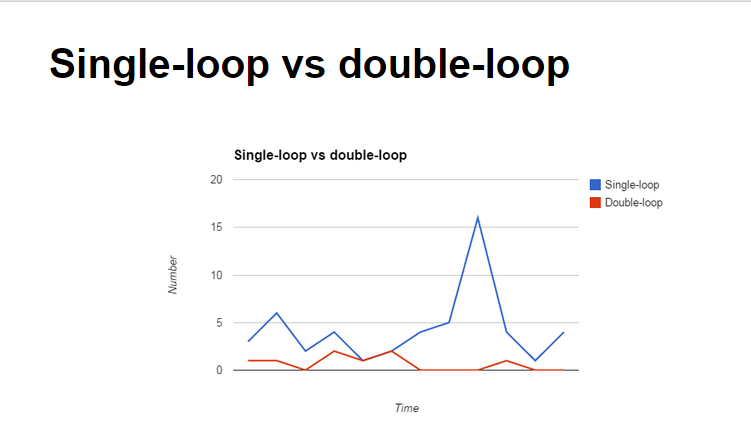
\includegraphics[width=\textwidth]{figures/Pilot_loop.PNG}
	\caption{An example of a slide from the pilot study presentation }
	\label{figure:Pilot Slide}
\end{figure}

\chapter{Content Analysis Categories}\label{appendix:categories}
The results of our pilot analysis gave us an extended set of categories that we will now describe further. Mainly we found six main themes that we could derive categories from. The six themes were: Nature, Context, Decision Making, Organizational Learning, Development and Management. We will describe each of these themes and their set of categories further in the sections below.

\section{Nature}
The nature of the action is the first theme that the content analysis is going to inspect. We define the nature of the action as how the origins of the action began. Did they come from a problem that occurred during the iteration or is it a continuation of something that has been working well in the past. Through our analysis we will try to understand the origins of the actions and classify them either as positive, negative or undefined. We define our classifications below. 
\paragraph{Positive} Positive actions is those actions where the origins of the action is in a positive context. If the action represents a current good working practice being continued, or something uncommon happened that gave positive results, it would be classified as positive.
\paragraph{Negative} The negative actions are those actions that has its origins from a problem or abnormal issue resulting in negative results. If an action is a result of a problem or abnormal issue it is classified as an negative action. 
\paragraph{Undefined} In the cases where it is unclear whether the origins of the action is positive or negative we classify the action as undefined. Such occurrences can be a result of missing context or actions that seem to have neither positive issues or negative issues as its origin. 

\section{Context}\label{method:context}
The context surrounding the action will be analyzed. The context off the action is based on the underlying issue that leads to the needed action. We divide the issues into three main categories, technical, process and undefined. 
\paragraph{Technical}
A technical issue can be a issue relating to technical competence, bugs or problems.
\paragraph{Process}
A process issue stems from a problem with a process, or potential for improvements in the existing processes. This can for example relate to communication between colleagues or work scheduling.
\paragraph{Undefined}
 An undefined issue might not have any clear origin, or might be too loosely described to be classified easily.

\section{Decision Making}
Rational decision making is how decision makers should think and should act based on coherence and rationality, according to M. Drury et al. ~\cite{Drury2012}. N.B. Moe et al. ~\cite{Moe2011} appends bounded rational decision-making as the means of understanding how decision making is made in non-routine activities. N.B. Moe et al. reasons that both are needed when analyzing decision-making in an agile context:
\begin{quote}
Software development involves both routine and non-routine activities. Hence, it makes sense to use both rational and bounded rational decision making theories when explaining decisions in software development processes. 
\end{quote}
Drury et al. distinguishes between two types of decisions being made in an organization, the strategic and the tactical. Moe et al. distinguishes between three types: Strategic, tactical and operational. We will use the three-type model. Each decision type will be described in the following paragraphs. 
\paragraph{Strategic}
A strategic decision is a wide ranging decision dealing with multiple or sizable issues, often causing major changes and have a long term impact.Moe et al. describes the strategic decisions as the following: 
\begin{quote}
Strategic decisions are related to organizational goals and objectives. The information concerning such decisions is usually incomplete and the decision-making process may extend over a considerable period of time.
\end{quote}
The actions that are categorized as strategical is the ones that proposes changes that have a long term impact or proposes changes that are related to the organizational goals. 
\paragraph{Tactical}
A tactical decision is smaller than a strategic decision it seeks to deal with the distribution and use of resources available to the team. Moe et al. described it as: 
\begin{quote}
Tactical decisions are related to identification and use of resources.
\end{quote}
All actions that specifically proposes to identification of resources or proposes changes to how resources are spent will be classified as tactical.
\paragraph{Operational}
Moe et al. describes an operational decision as: 
\begin{quote}
Operational decisions deal with ensuring effectiveness of day-to-day operations within the organization. 
\end{quote}
Every action that are restricted to only day-to-day operations will be classified as operational decisions. They might be quick fixes that solve a single problem. 
\paragraph{Undefined}
An undefined decision might be difficult to categorize because of a lack of context or an unclear description.

\section{Organizational Learning}
Organizational learning is a process where an organization takes steps to improve its current work environments by reacting to issues that arise. These steps can be varied, and we divide them into single-loop, double-loop and undefined. Retrospectives have a central role in 	organizational learning, as described by Dingsøyr ~\cite{Dingsoyr2007}
\paragraph{Single-loop}
A single-loop action is an action designed to change or tune a process in order to improve it. The action does not seek to address underlying problems, and are a single-feedback loop from observing an issue to making a change. A retrospective can facilitate single-loop learning where the project team uses the input during the retrospective to make adjustments to their current work ~\cite{Dingsoyr2004}
\paragraph{Double-loop}
A double-loop action is designed to solve an issue, as well as address the underlying cause of the issue. This requires an understanding of the underlying issue and the nature of its influence. Double-loop decisions can be facilitated through a retrospective, often these are as a result of a more drastic need for change and an understanding of the underlying problem. ~\cite{Dingsoyr2004}
\paragraph{Undefined}
An action might not be clearly described, or the nature of the action can not be interpreted. We will classify these actions as undefined.

\section{Development}
An issue that is related to the development of the product is included in this category. The development process is the actual work performed to create the product, as well as processes directly related to this work. The different categories included in development were chosen after discussing with advisors, as well as personal experience from the writers
\paragraph{Development}
Development includes the writing of code, specifying requirements, construction the system architecture and other aspects of designing of the system. 
\paragraph{Planning}
An action that is categorized as planning is when the action is suggesting changes to planning in future iterations or is a result of an issue occurring in a former iteration. Estimations, task-prioritization, scheduling and etc. all goes under the planning category.
\paragraph{Testing}
Issues related to the testing of a product, this includes unit, module and system testing. Issues related to testing can also be communication between testers and developers.
\paragraph{Documentation}
Action that are categorized as documentation is those that are related to the documentation part of developing a system. Typical actions are those that describe or propose changes to documentation practices. This can also include tutorials that explains the product and improves usability. 
\paragraph{Builds}
During development of a software system building the software system can be a tiresome task. The actions that are categorized as builds are those who proposes practices that changes the current build practices.
\paragraph{Release}
When a system feature or a part of a system is finished, usually at the end of an iteration, one deploy the new part of the system into production, available for the users. For the actions that categorized as release, the action describe some aspect of the release practice and either proposes changes or suggest new practices.
\paragraph{Business}
Business development is a critical part for an organization to create profit. Software system often can save costs and create new business opportunities and as a part of a software development team one also has to consider business perspectives. We categorize all actions that are related to business development or proposes some business related changes as business. 
\paragraph{Undefined} If an action is neither of the development phases described above we classify it as undefined. 

\section{Collaboration}
One of the aspects during a software developing process is collaboration. Fægri ~\cite{Faegri2012} describes collaboration as the following: 
\begin{quote}
Collaboration is a key aspect of software development. Collaboration allows groups of software practitioners to deal with uncertainty, complexity and interdependence. And in dealing with these challenges, the group demonstrates its collective problem-solving ability.
\end{quote}
Through our pilot analysis we registered several activities that are related to collaboration. Communication, leadership, competence, external relations and planning all belongs beneath the collaboration banner, and we describe in detail how we classify each of them below. 
\paragraph{Communication}
Communication is a widely used word and concept, but it rarely is defined. By using Merriam-Webster dictionary ~\cite{MerriamWebster2015} we found a definition that can serve as a clarification: 
\begin{quote}
The act or process of using words, sounds, signs, or behaviors to express or exchange information or to express your ideas, thoughts, feelings, etc., to someone else.
\end{quote}
Nakakoji et al. ~\cite{Nakakoji2010} distinguishes between two types of communication related to software development, coordination communication and expertise communication. The first one being the process of coordinating the development activities and the last one being when a developer obtain some information regarding a software artifact, either through code comments, wikis or other means. 
We are however not going to distinguish between these two communication types in our content analysis as we believe the two differentiations is covered by the context of the action as described in \autoref{method:context}. For our content analysis we are simply going to count every instance of communication for every action that is related to communication between team-members regardless if it is through text, speech or other means of communication.
\paragraph{Leadership}
As is the case with communication, leadership is also widely used concept, that is rarely specified. Again we turn to Merriam-Webster \cite{MerriamWebster2015} for a definition: 
\begin{quote}
The power or ability to lead other people.
\end{quote}
Agile development teams is often self-organized as it is one of the principles in the agile manifesto \cite{AgileManifesto2015}. This can result in no clear leadership. For our content analysis we are going to consider decisions and guidelines set by the group itself as leadership activities. We categorize actions as leadership if they somehow suggests changes to leadership or if the actions is a result of some leadership related issue. 
\paragraph{Competence}
We define competence as the ability to perform a certain task in a adequate quality. Each member within an agile team has their own set of knowledge that they use to solve different tasks. If any issues arises and the group is lacking the knowledge to counter it we categorize the action created to resolve it as an competence action. An example could be issue of lacking the knowledge resolving a database error and the action is to send one developer at a database course. This action would then be categorized as an competence action.
\paragraph{External Relations}
By the category external relations we mean if the team has any actions that is a result of issues arising from external factors or the actions that team is creating to inflict some external factors. Example of external relations can be customer relations, communication with server maintenance team or other development teams.   
\paragraph{Undefined}
For those actions that the origin is unclear and the goal is not related to any of the collaboration categories we categorize them as undefined.

\chapter{Shared Mental Models}
\label{section:mental-models}
The theory of shared mental models is from cognitive psychology, and can be used as a lens to evaluate agile development and methodology as described by Petter et al\cite{Petter2013}. The concept is that a team has a shared mental model that is central to the mutual understanding between team members, and thus essential to project success. Without a good shared mental model a team is left with a poor understanding of the task at hand, as well as barriers for cooperation. Two metrics used to measure a team's shared mental model are ``similarity'' and ``accuracy''. Where ``similarity'' is the degree which the shared mental model is similar between team members, and ``accuracy'' is the degree which the shared mental model matches objective measures. 

\section{The stages of Shared Mental Model generating}

\label{section:mental-models-stages}
	
Four different stages of building shared mental models are identified \cite{Petter2013}. These are knowing, learning, understanding and executing. An overview of these stages is seen in  \autoref{table:stages-mental-model}. Knowing is the stage where a team gets exposed to information relating to their project and project goals, at this stage team members are encouraged to share information between each other. The second stage is the learning stage, this stage consists processing the information gained in the knowing stage. The understanding stage is defined by reaching consensus and understanding the team member's individual views. Executing is the last stage, with a developed shared understanding the team is able to reach goal, at this stage a team responds to a situation based on the work done in the previous stages.

\begin{table}[!h]
	\begin{centering}
	\caption{Four stages of mental model building}
	\label{table:stages-mental-model}
	\begin{tabular}{l | p{0.7\textwidth}}

	\hline
	Stage & Description \\
	\hline
	Knowing &  Information exposure and sharing\\
	Learning & Information processing \\
	Understanding & Consensus and common ground \\
	Executing & Shared understanding and  \\
	\hline
	
\end{tabular}
\end{centering}
\end{table}

	
\section{Shared Mental Models and retrospectives}

Petter et. al. \cite{Petter2013} describe multiple agile development practices, but do not focus a lot on the agile retrospective. In the appendix of the article they give the following link between retrospectives and shared mental models.

\begin{quote}
Enhances the development of learning and understanding stages by facilitating the information sharing and integration. This practice also improves the teams’ executing capability in the next sprint
\end{quote}

The shared mental model practices that are involved in the retrospective are identified as self corrective, training and reflectivity. We discuss the relationship between our results, retrospectives and shared mental models in \autoref{section:shared-mental-models-discussion}.


\section{Shared mental models discussion}
\label{section:shared-mental-models-discussion}
In \autoref{section:mental-models} we describe the basics of the shared mental models theory and its relation to agile development. In this section we will see how agile retrospectives can impact the four stages of shared mental model generation described in \autoref{section:mental-models-stages}. Our thoughts are a result of the analysis and interviews. It should be noted that the agile retrospective described in Petter et al. \cite{Petter2013} confines the retrospective to being in the end of a sprint, while our work does not put the same confines on the retrospective.

\paragraph{Improves Shared Mental Model}
The knowing stage is not included in the domain of the sprint retrospective described by Petter et al. \cite{Petter2013}, in our work we found that the facet of team members sharing their individual knowledge, thereby updating the shared information. One example of this was found in team Echo, where the different sub teams would use the retrospective to share their discoveries and knowledge development, thus updating the meta-knowledge of the team as a whole. 

The learning phase of the shared mental model is impacted by the agile retrospective by using techniques that facilitate the integration of the knowledge from the knowing stage. One example could be the use of evidence based time lines as described by Bjarnasson et al. \cite{Bjarnason2012}, where the time line would work as an outline of the information received by the team. Another example is seen in the weekly retrospectives held by team Delta, where team members would continually update their colleagues on their work day, allowing for reflexivity. Another example would be the use of the ``five times why''-technique as used by team Charlie and Echo, where both the possibility for reflexivity and self correction exists.

The understanding phase described by Petter et al. \cite{Petter2013} is far reaching and includes many facets of team cooperation and some of them are described in \autoref{section:mental-models-stages}. One part of the understanding phase we did not expect to see explicitly in our study was conflict resolution on a personnel level, and can be considered part of the conflict reconciliation and consensus building that is part of the understanding phase. Also part of the understanding phase is the practice of refining team communication and team processes which is a central component of the retrospective purpose. We observed every team discussing these topics during our interviews and analysis. Lastly, not included in the work of Petter et al. is the use of the retrospective as a tool for planing, and 24.6 percent of the actions analyzed in our work with team Zulu were deemed to have a planning component, as described in \autoref{section:development-phase}. This planning component could be said to be increasing the similarity of the information between team members.

The execution is perhaps the phase most impacted by the retrospective, as the explicit actions decided during a retrospective almost always is intended to improve or refine the processes that in one way or another help them reach their goals. For example the information similarity generated in the understanding phase can lead to a quicker response time to new tasks. One typical example is the refining of the communication processes as seen in team Zulu, or the introduction of the bug-fix days described in \autoref{section:bugfix}. 

\paragraph{Shared Mental Models Practice}
In this section we discuss observations on the relationship between retrospectives and shared mental model practices.

Reflectivity is a central part of the learning process in the team. We have observed that many teams use the retrospective as a review tool of the last work period. We have observed very different practices when it comes to frequency as seen in \autoref{table:frequency-duration}, and thus the definition of a work period is different from the sprint retrospective definition from Petter et al. One observation done by us is that very few teams practice reflectivity on the retrospective itself, or if they do they do not formally do it on the team level, as seen in team Charlie. In team Charlie the scrum master would discuss and reflect on the retrospective with other scrum masters and team leaders within the company, but it would not be brought back to the team. In some ways the analysis done with team Zulu together with the feedback sessions with them could potentially be considered an example of this kind of reflectivity. The interviews done with team Zulu's leader and SCRUM master suggests that both the team's mental model similarity and accuracy was improved through the analysis and reflection done.

The sprint retrospective defined by Petter et al. Does not include planning, but our work with team Zulu indicates that planning is an integral part of retrospective actions in some teams. This is discussed in \autoref{section:development-phase}, this high degree of presence of planning was unexpected and more thought on the potential of mental model improvement through planning in retrospective seems interesting. For example the use consensus based approach used by team Golf in planning could potentially increase the similarity of the team's mental model.

\chapter{Graphs of Results from Content Analysis}
\label{appendix:graphs}
\begin{figure}[!h]
	\centering
	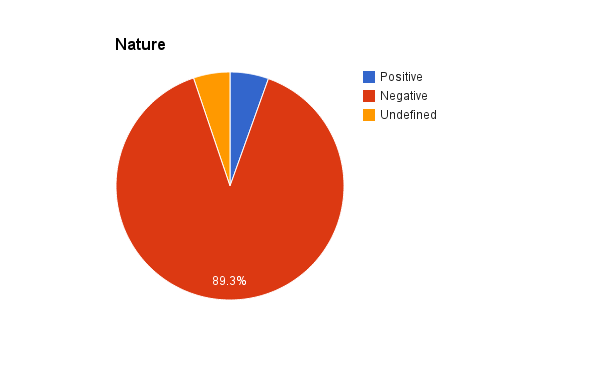
\includegraphics[width=\textwidth, keepaspectratio]{figures/nature-p.png}
	\caption{The negative, positive and undefined distribution of all the actions.}
	\label{figure:nature-p}
\end{figure}

\begin{figure}[!h]
	\centering
	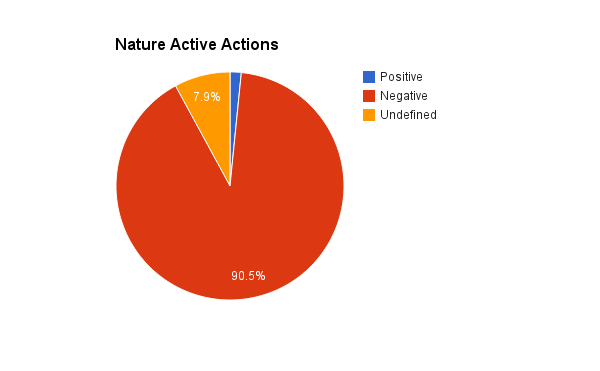
\includegraphics[width=\textwidth, keepaspectratio]{figures/nature-pa.png}
	\caption{The negative, positive and undefined distribution of the active actions.}
	\label{figure:nature-pa}
\end{figure}

\begin{sidewaysfigure}[!h]
	\centering
	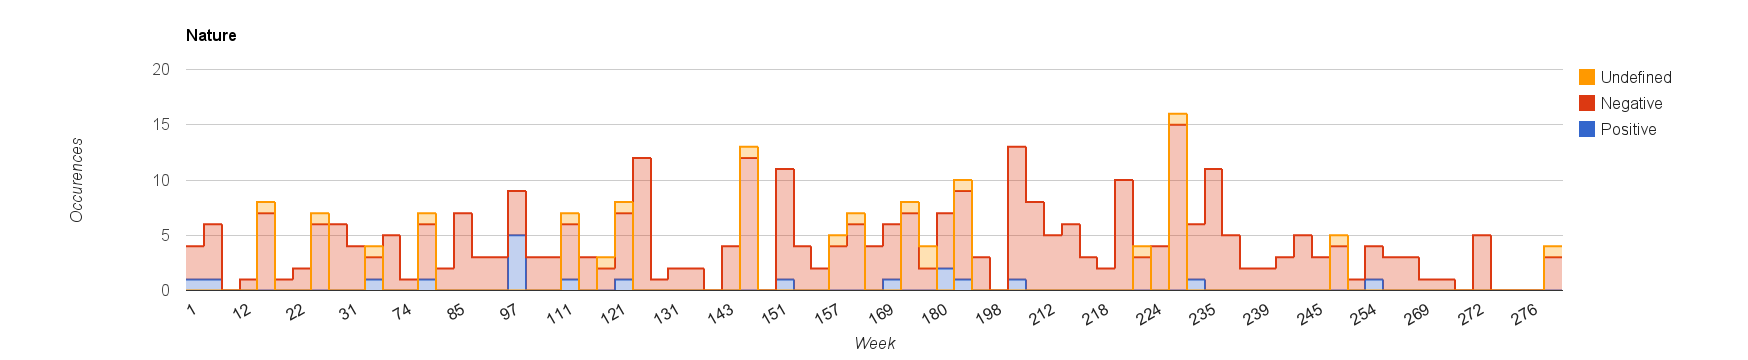
\includegraphics[width=\textwidth, keepaspectratio]{figures/nature-l.png}
	\caption{The distribution of negative, positive and undefined actions across the timespan}
	\label{figure:nature-la}
\end{sidewaysfigure}

\begin{figure}[!h]
	\centering
	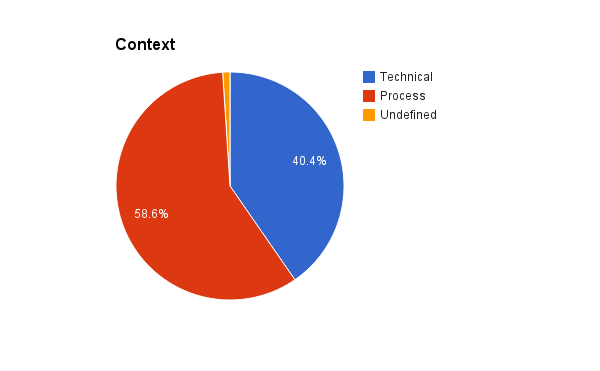
\includegraphics[width=\textwidth, keepaspectratio]{figures/context-p.png}
	\caption{The distribution of technical, process and undefined related actions.}
	\label{figure:context-p}
\end{figure}

\begin{figure}[!h]
	\centering
	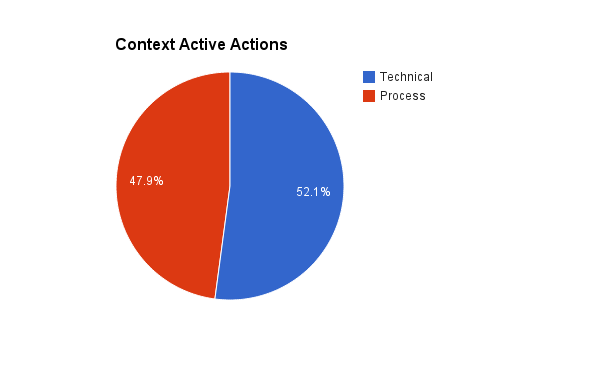
\includegraphics[width=\textwidth, keepaspectratio]{figures/context-pa.png}
	\caption{The distribution of technical, process and undefined related actions over.}
	\label{figure:context-pa}
\end{figure}

\begin{sidewaysfigure}[!h]
	\centering
	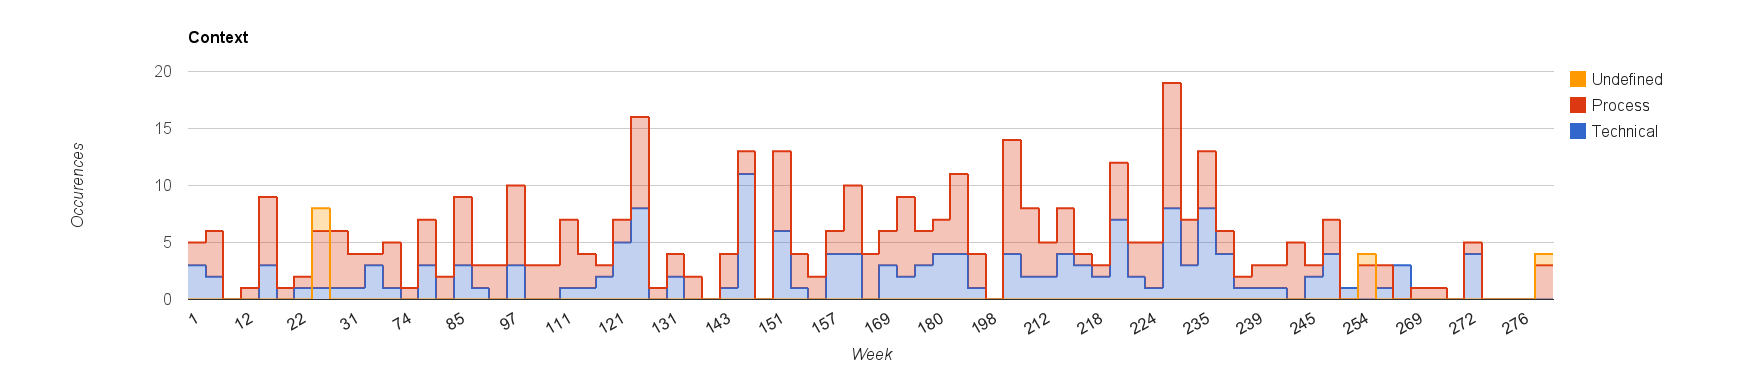
\includegraphics[width=\textwidth, keepaspectratio]{figures/context-l.png}
	\caption{The distribution of technical, process and undefined related actions across the timespan.}
	\label{figure:context-la}
\end{sidewaysfigure}

\begin{figure}[!h]
	\centering
	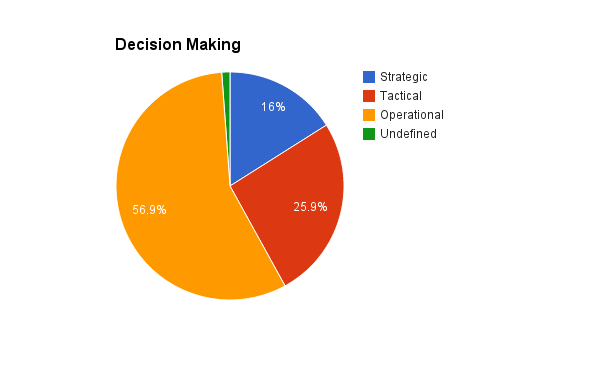
\includegraphics[width=\textwidth, keepaspectratio]{figures/decision-p.png}
	\caption{The distribution of different decision making decisions as they occurred over all the actions.}
	\label{figure:decision-p}
\end{figure}

\begin{figure}[!h]
	\centering
	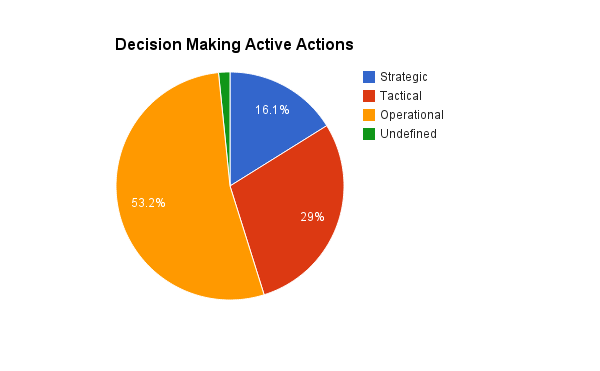
\includegraphics[width=\textwidth, keepaspectratio]{figures/decision-pa.png}
	\caption{The distribution of different decision making decisions as they occurred over the active actions.}
	\label{figure:decision-pa}
\end{figure}

\begin{sidewaysfigure}[!h]
	\centering
	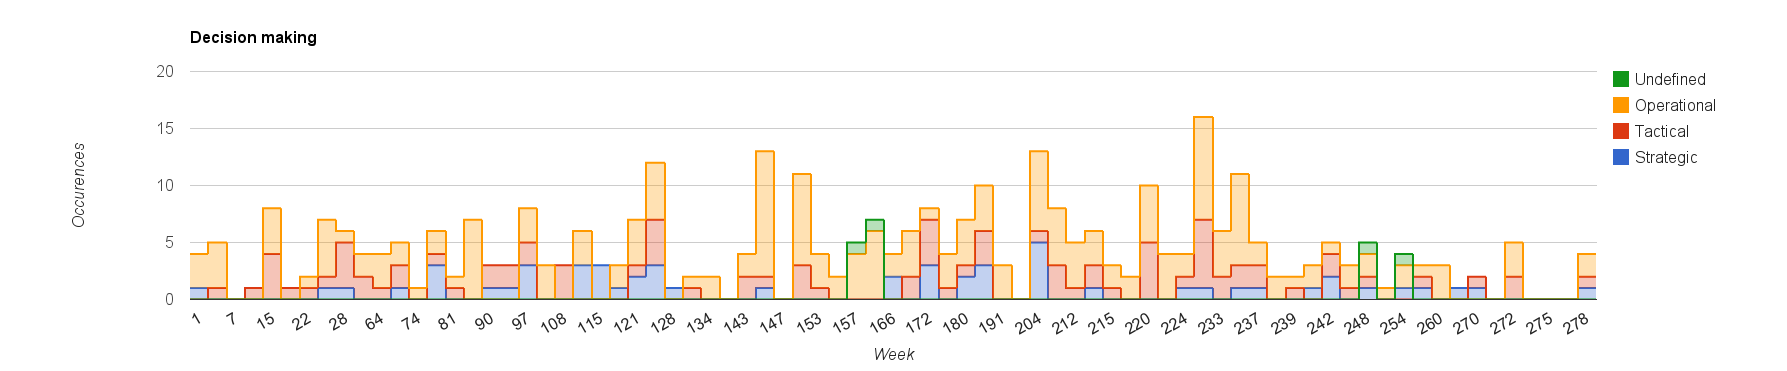
\includegraphics[width=\textwidth, keepaspectratio]{figures/decision-l.png}
	\caption{A timeline showing the distribution of the different decision making decisions for all the actions.}
	\label{figure:decision-la}
\end{sidewaysfigure}

\begin{figure}[!h]
	\centering
	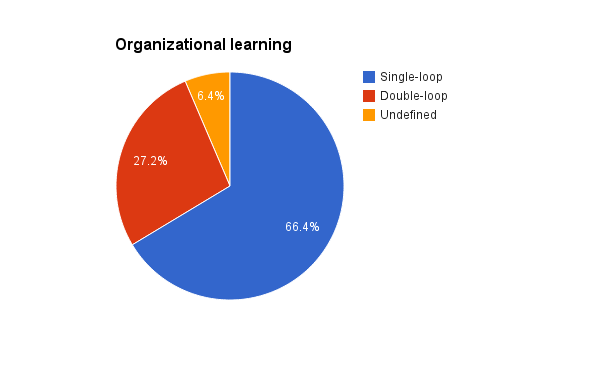
\includegraphics[width=\textwidth, keepaspectratio]{figures/learning-p.png}
	\caption{The distribution of single-loop, double-loop and undefined for all the actions.}
	\label{figure:learning-p}
\end{figure}

\begin{figure}[!h]
	\centering
	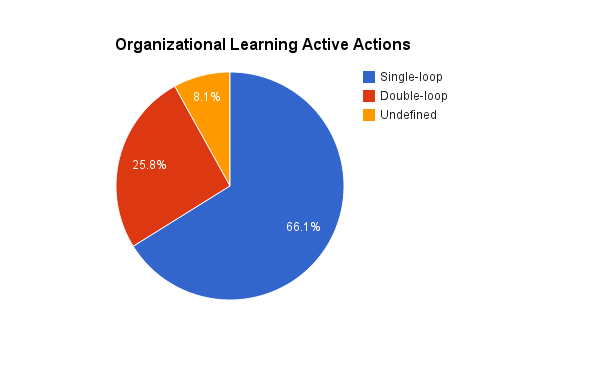
\includegraphics[width=\textwidth, keepaspectratio]{figures/learning-pa.png}
	\caption{The distribution of single-loop, double-loop and undefined for the active actions.}
	\label{figure:learning-pa}
\end{figure}

\begin{sidewaysfigure}[!h]
	\centering
	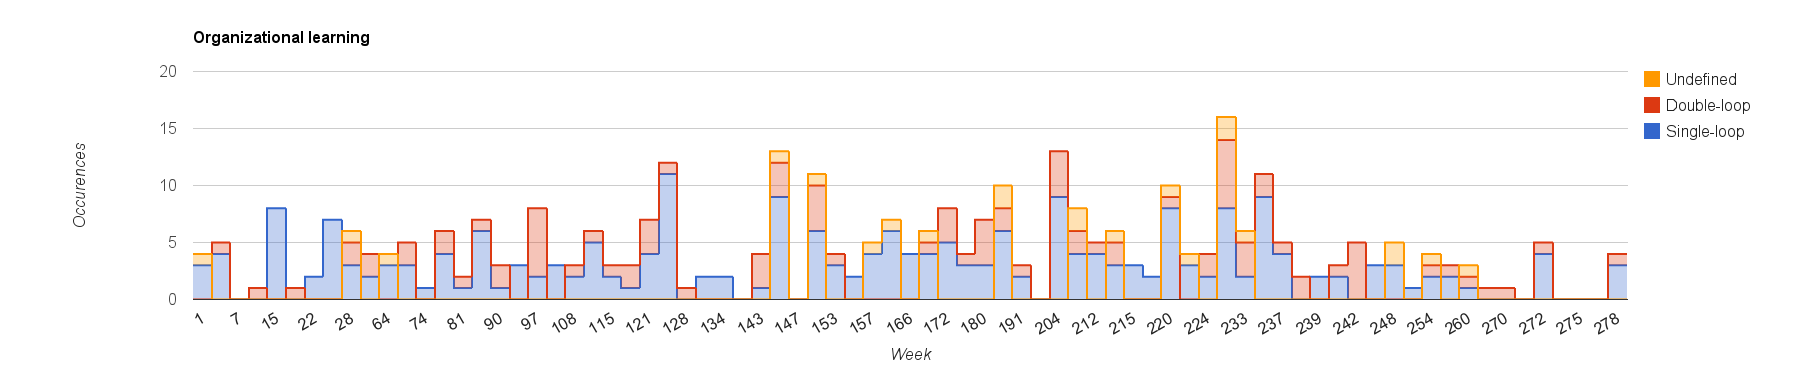
\includegraphics[width=\textwidth, keepaspectratio]{figures/learning-l.png}
	\caption{Timeline showing the distribution of learning loops for the total actions.}
	\label{figure:learning-la}
\end{sidewaysfigure}

\begin{figure}[!h]
	\centering
	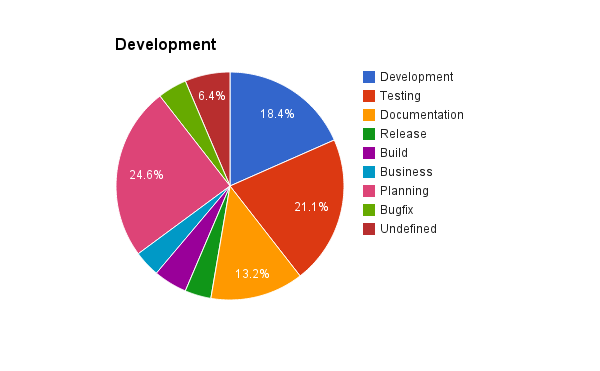
\includegraphics[width=\textwidth, keepaspectratio]{figures/development-p.png}
	\caption{The distribution of the different development phases for all the actions.}
	\label{figure:development-p}
\end{figure}

\begin{figure}[!h]
	\centering
	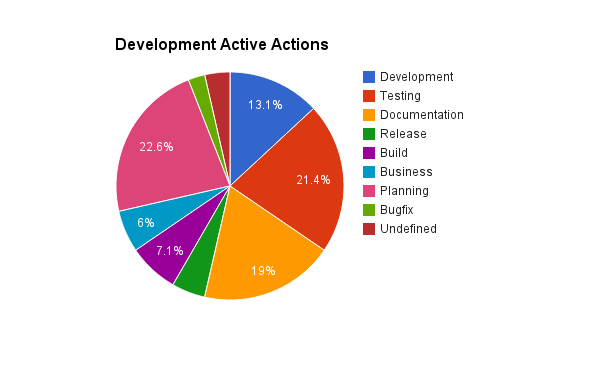
\includegraphics[width=\textwidth, keepaspectratio]{figures/development-pa.png}
	\caption{The distribution of the different development phases for the active actions.}
	\label{figure:development-pa}
\end{figure}

\begin{sidewaysfigure}[!h]
	\centering
	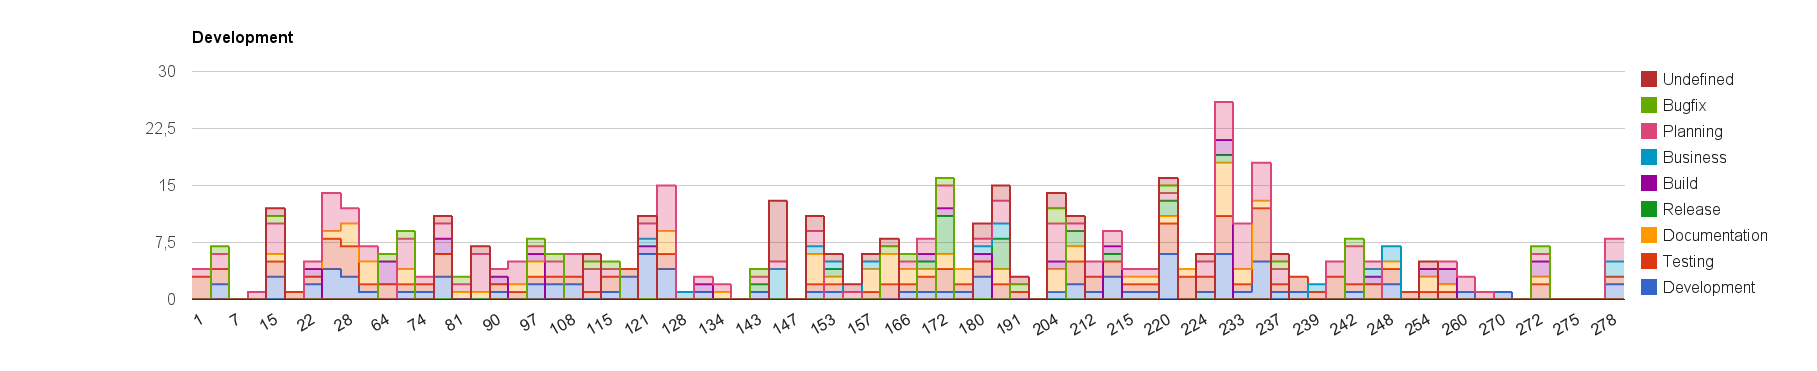
\includegraphics[width=\textwidth, keepaspectratio]{figures/development-l.png}
	\caption{Timeline showing the distribution of the different development phases over time.}
	\label{figure:development-la}
\end{sidewaysfigure}

\begin{figure}[!h]
	\centering
	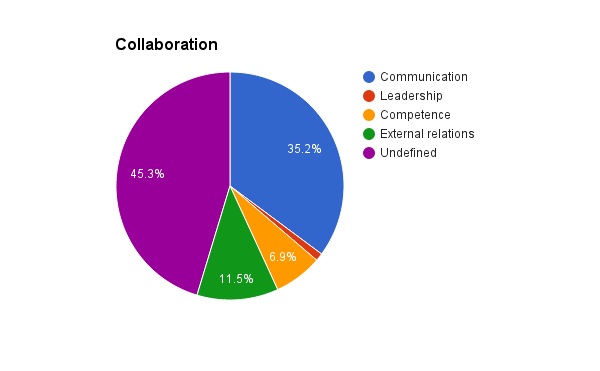
\includegraphics[width=\textwidth, keepaspectratio]{figures/management-p.png}
	\caption{The distribution of different collaboration categories for all the actions.}
	\label{figure:learning-p}
\end{figure}

\begin{figure}[!h]
	\centering
	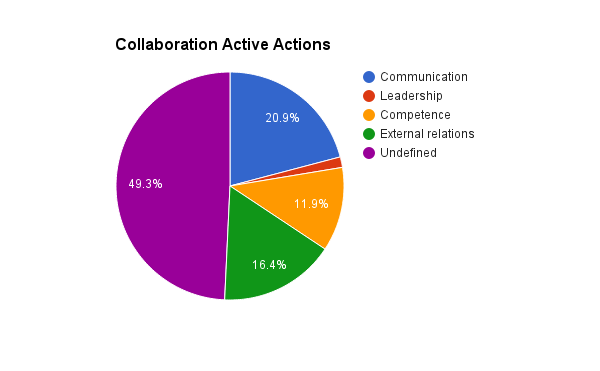
\includegraphics[width=\textwidth, keepaspectratio]{figures/management-pa.png}
	\caption{The distribution of different collaboration categories for the active actions.}
	\label{figure:learning-pa}
\end{figure}

\begin{sidewaysfigure}[!h]
	\centering
	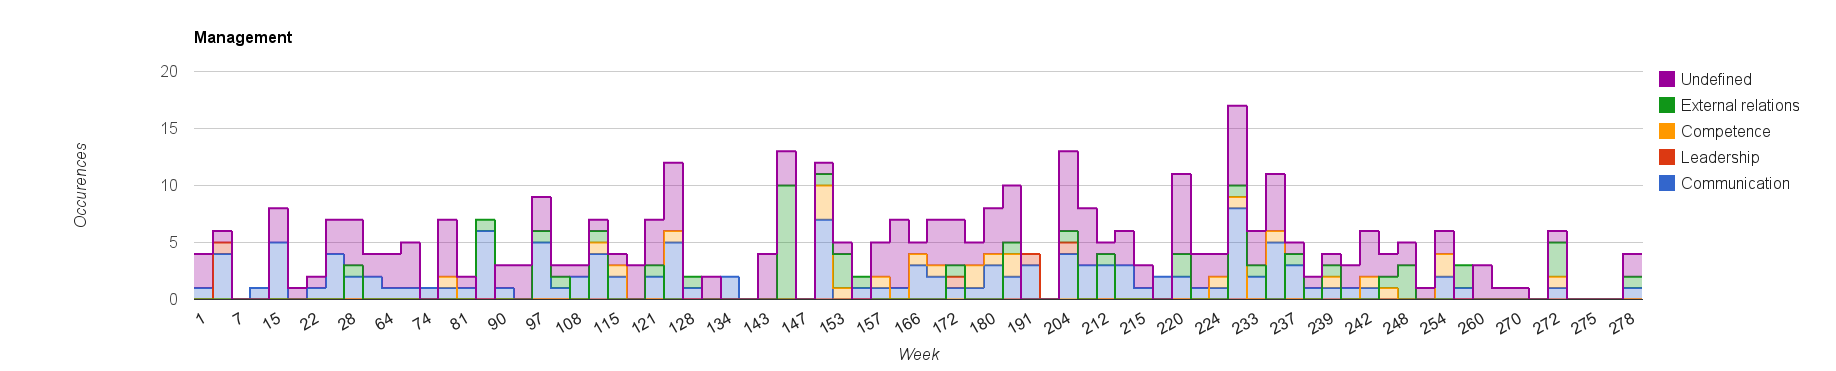
\includegraphics[width=\textwidth, keepaspectratio]{figures/management-l.png}
	\caption{Timeline showing the distribution of the different collaboration categories over time.}
	\label{figure:learning-la}
\end{sidewaysfigure}



